\documentclass[a4paper,11pt]{article}
\usepackage[T1]{fontenc}      % codifica dei font
\usepackage[utf8]{inputenc}
\usepackage[italian]{babel}
\usepackage{lipsum}
\usepackage{comment}
\usepackage{url}
\usepackage{amsfonts}
\usepackage{graphicx}
\begin{document}
% lettere accentate da tastiera
% lingua del documento
% genera testo fittizio
% per scrivere gli indirizzi Internet
\author{Linpeng Zhang}
\title{Tutorato AFL}
\maketitle
\begin{abstract}
    Per errori/dubbi/problemi: linpeng.zhang@studenti.unipd.it.
\end{abstract}
\tableofcontents
\section{Lez10}
\subsection{Esercizi}
\begin{enumerate}
    \item Convertire in CNF la seguente grammatica:\\
    $S\rightarrow aAa|aa|bBb|bb$\\
    $A\rightarrow C|a$\\
    $B\rightarrow C|b$\\
    $C\rightarrow CDE|DE|CE|E$\\
    $D\rightarrow A|B|ab$\\
\end{enumerate}
\subsection{Soluzioni}
\begin{enumerate}
    \item \begin{enumerate}
    \item eliminiamo i simboli non generatori: dunque C,E\\
    $S\rightarrow aAa|aa|bBb|bb$\\
    $A\rightarrow a$\\
    $B\rightarrow b$\\
    $D\rightarrow A|B|ab$\\
    \item eliminiamo i simboli non raggiungibili: D\\
    $S\rightarrow aAa|aa|bBb|bb$\\
    $A\rightarrow a$\\
    $B\rightarrow b$\\
    \item elimino le $\epsilon$ produzioni che in questo caso non ci sono
    \item trovo le coppie unitarie: non ce ne sono;
    \item     $S\rightarrow AAA|AA|BBB|BB$\\
    $A\rightarrow a$\\
    $B\rightarrow b$\\
    \item     $S\rightarrow AC|AA|BD|BB$\\
    $A\rightarrow a$\\
    $B\rightarrow b$\\
    $C\rightarrow abSca$\\
    $D\rightarrow BB$\\
    \end{enumerate}
\end{enumerate}
\subsection{Traccia alle risposte delle domande della simulazione}
\begin{enumerate}
    \item si dimostra per induzione sul numero di derivazioni; con una derivazione si deriva $\epsilon$ che banalmente soddisfa la proprietà; con $n+1$ derivazioni, dopo la prima si ha $aS$ oppure $aSbS$ e con altre n derivazioni si ha $aw'$ oppure $aw'bw''$ con $w', w''$ che soddisfano la proprietà. Naturalmente anche $aw'$ la soddisfa (visto che si aggiunge una a all'inizio) e lo stesso per $aw'bw''$, visto che si aggiunge una a all'inizio e una b che è matchata dalla a aggiunta all'inizio;
    \item \begin{minipage}{\linewidth}
        $\delta (q, \epsilon, S) = \{(q,aS), (q,aSbS), (q, \epsilon)\}$\\
        $\delta (q, a, a) = \{(q,\epsilon)\}$\\
        $\delta (q, b, b) = \{(q,\epsilon)\}$\\
    \end{minipage}
    \item un DPDA che accetta per stati finiti riconosce tutti i linguaggi regolari (basta ignorare lo stack), ma non tutti i CFL: ad esempio $ww^r$ no e un esempio è data dalle stringhe $0110$ e $01100110$. L'automa deterministico dopo aver letto la prima stringa (che dovrebbe accettare) deve aver consumato lo stack (prima mette 01 in pila poi leggendo 10 matcha lo stack). Ma allora se leggesse 01100110 come si dovrebbe comportare? Avrebbe già svuotato lo stack consumando solo metà input!\\
    Un DPDA che accetta per stack vuoto accetta solo linguaggi accettati da DPDA che hanno la proprietà del prefisso. L'intuizione è simile: se il DPDA legge x, deve averlo consumato. Quindi non può leggere x seguito da qualcos'altro, ovvero deve esserci sempre la proprietà del prefisso.\\
    Importanza: si è dimostrato che se un DPDA riconosce un linguaggio, allora tale linguaggio non è inerentemente ambiguo.
    \item è chiaro che l'automa non svuoti mai la pila, quindi si presume che riconosca per stato finale. Quando legge una a la mette in cima. Quando legge una b, se c'è una a in cima la toglie, altrimenti si blocca (non ha transizioni). Quindi si può intuire che l'automa riconosca l'insieme delle stringhe per cui ogni prefisso ha un numero di a maggiore o uguale al numero di b. Usare la costruzione vista a lezione per la conversione.
    \item (a): il consiglio presente nella consegna vi dice già come risolvere l'esercizio. Caso base: 1 derivazione, si deriva la stringa $\epsilon$ che è banalmente bilanciata. Con n+1 derivazioni, la prima può usare una delle due produzioni. Seguono n derivazioni, che portano ad avere o la concatenazione di due stringhe bilanciate o del tipo $(w)$ con w bilanciato. Naturalmente in entrambi i casi la proprietà è rispettata e si ha la tesi.
    \\(b): non genera ad esempio $()()$.
    \item \begin{minipage}{\linewidth}
        $[qXq] \rightarrow a[qYq][qZq]$\\
        $[qXq] \rightarrow a[qYp][pZq]$\\
        $[qXp] \rightarrow a[qYq][qZp]$\\
        $[qXp] \rightarrow a[qYp][pZp]$\\
    \end{minipage}
    \item basta applicare la costruzione per rimuovere $\epsilon -$produzioni; in particolare le variabili annullabili sono $Z=\{S\}$. Sostituiamo ad ogni occorrenza di S, la possibilità che questo ci sia o meno.\\
    $S\rightarrow ASB|AB$\\
    $A\rightarrow aAS|aA|a$\\
    $B\rightarrow bS|Sb|b|SbS|A|bb$\\
    \item non fatto;
    \item se una grammatica ha h simboli, allora una parola w lunga almeno $2^h$ richiederà che due simboli si ripetano nell'albero di derivazione. Sia A il simbolo che si ripete, allora l'albero radicato in A deriva o xAy o w. Chiaramente si può ripetere "xAy" infinite volte. Si ha quindi il PL.
     \item risolto in lez9;
     \item è immediato scrivere una CFG che riconosce questo linguaggio: $S \rightarrow abSca\ |\ abca$. La conversione è altrettanto immediata. L'automa ottenuto è nondeterministico, ma si potrebbe anche scriverne uno deterministico: l'idea è  il DPDA possa cominciare il matching dopo aver letto la c. Si noti inoltre che vale la regola del prefisso (ciò non garantisce che esista un DPDA che riconosca tale linguaggio. Ma se non valesse, allora certamente non esisterebbe un DPDA per stack vuoto che accetti tale linguaggio);
     \item $L_u = \{ (M,w)\ | \ M$ è una $TM$ con input 0/1, $w$ è una stringa di 0/1 e $w \in L(M)\}$.\\Certamente $L_u$ è RE: infatti basta simulare M su w.
     \\Se $L_u$ fosse ricorsivo anche $comp(L_u)$ lo sarebbe. Ma se avessimo una TM per $comp(L_u)$ si potrebbe utilizzare tale TM per riconoscere $L_d$, il che porterebbe a una contraddizione. La riduzione è semplice: presa un'istanza $w$ per $L_d$, proviamo $(w,w)$ sulla TM $M$ che riconosce $comp(L_u)$. Se $M$ accetta $(w,w)$, allora la $TM$ codificata da $w$ non accetta $w$, quindi l'istanza iniziale $w$ appartiene a $L_d$. Analogo il caso "rifiuta".
     \item Una TM multi track è fatta da un singolo nastro a cui corrisponde ad ogni cella un certo numero di simboli indipendenti tra di loro. Una TM multinastro è formata da più nastri infiniti e si ha una testina su ogni nastro. In particolare la TM può controllare tutte le testine e fare un passo. La simulazione di n passi ha costo $O(n^2)$: la TM mononastro per simulare k nastri deve avere 2k tracce: su k tracce mette i simboli dei nastri, sulle altre segna eventualmente la presenza di testine. Quando la TM multinastro compie n passi, per ogni passo la TM mononastro deve spostarsi di $O(n)$ passi. Quindi per svolgere n passi impiegherà tempo quadratico: $O(n^2)$.
     \item $L_e = \{M|L(M)=\emptyset\}$.\\
     $L_{ne} = \{M|L(M)\neq \emptyset\}$\\
     $L_{ne}$ è RE: basta provare non deterministicamente tutti gli input con la TM universale. Inoltre $L_{ne}$ non è ricorsivo: infatti possiamo ridurre $L_u$ a $L_{ne}$: basterà costruire una TM che, presa un'istanza $x=(M,w)$ per $L_u$, passi come input alla TM per $L_{ne}$ un'istanza $h(x)$ che rappresenta una $TM$ che ignora l'input e simuli $M$ su $w$. $L_e$ non è RE: se lo fosse, allora essendo $L_e=$comp$(L_{ne})$ si avrebbe che $L_e, \L_{ne}$ sono ricorsivi: ma allora si avrebbe un assurdo con la dimostrazione precedente.
    
     %   \item si può dimostrare che A genera $L_A=\{a^nb^m|n=m+1$ oppure $n=m$ con $n>0,m\geq 0\}$, B genera $L_B=\{a^nb^m|m=n+1$ oppure $n=m$ con $m>0,n\geq 0\}$. Dalle due asserzioni precedenti si dimostra che S genera $L_S=\{a^nb^m|n=m+1$ oppure $n=m$ con $n,m>0\}$: infatti S produce le stringhe che produce B con una a all'inizio, e la correttezza segue dalla definizione.\\
   %  Un automa a pila che accetta tale linguaggio è:\\
  %  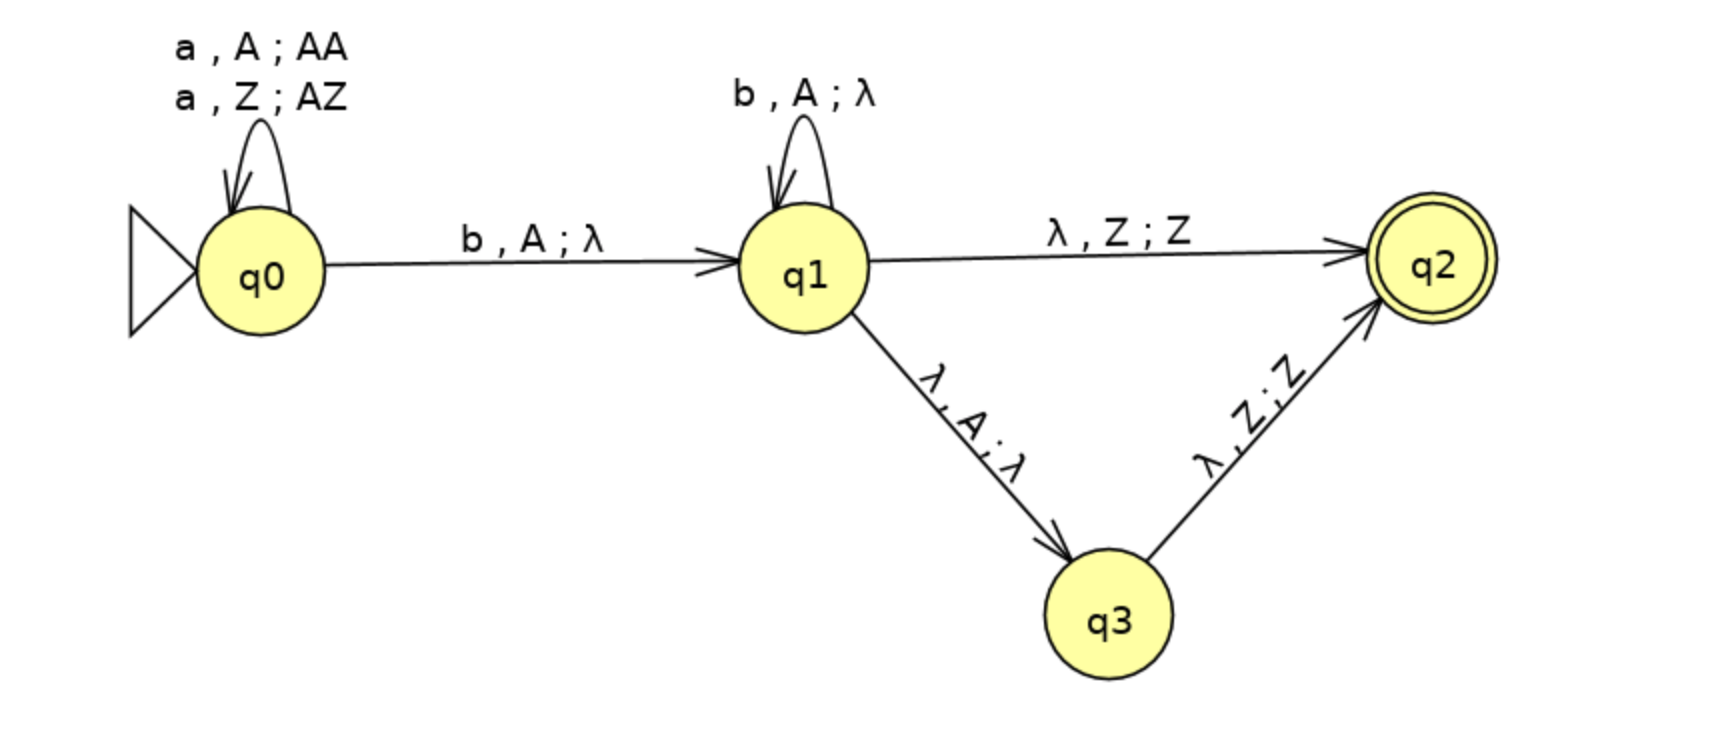
\includegraphics[scale=0.5]{Lez7sol6.png}
\end{enumerate}

\begin{comment}
          \item \begin{minipage}{\linewidth}
        $S \rightarrow [qZq]$\\
        $(1) [qZq] \rightarrow 1[q1q][qZq]$\\
        $(2) [qZq] \rightarrow 0[q0q][qZq]$\\
        $(3) [q1q] \rightarrow 0$\\
        $(4) [q0q] \rightarrow 1$\\
        $(5) [q1q] \rightarrow 1[q1q][q1q]$\\
        $(6) [q0q] \rightarrow 0[q0q][q0q]$\\
        $(7) [qZq] \rightarrow \epsilon$\\
      \end{minipage}
       \item Sia data la CFG:\\
     \begin{minipage}{\linewidth}
        \centering $S \rightarrow aB$\\
        \centering $B \rightarrow Ab\ |\ b$\\
        \centering $A \rightarrow aB\ |\ a$\\
    \end{minipage}
    \\Dire: linguaggio accettato e definire un automa che accetti tale linguaggio.
\end{comment}
    % Bibliografia
    %\begin{thebibliography}{9}
        %  Alcune soluzio
    %\end{thebibliography}
    \end{document}